\documentclass[a4j,twocolumn]{jsarticle}

\usepackage[dvipdfmx]{graphicx}

\setlength{\textheight}{275mm}
\headheight 5mm
\topmargin -30mm
\textwidth 185mm
\oddsidemargin -15mm
\evensidemargin -15mm
\pagestyle{empty}

\begin{document}
\title{Mg-LPSOのL1$_2$クラスターの第一原理計算}
\author{情報科学科 西谷研究室 3539 山本 泰基}
\date{}
\maketitle
\section{背景}
LPSO ( Long Period Stacking Order )構造をもったMgは比降伏強度でジュラルミンを上回る特性を持ち,
かつ難燃性であるため次世代の航空機の構造材料として実用化が始まっている.
LPSO構造を図 1 に示した\cite{kiyohara}. 
西谷研究室では,このLPSO構造の生成機構として「積層欠陥部に L1$_2$クラスターが形成され,そこから排斥された Zn, Yが,濃化して新たなL1$_2$クラスターを形成する」というシナリオを立て\cite{sakamoto},
第一原理計算を用いて系のエネルギーからそのシナリオの実現性を評価してきた. 
第一原理計算は,量子力学を支配するシュレディンガー方程式を精確に解いて, 原子の種類だけから電子構造を求め, いろいろな物性を予測する計算である. 
計算の結果, 系全体のエネルギーは溶質原子とL1$_2$クラスターとの距離が離れるにつれ単調に減少し安定となったが, それは中周期的に溶質原子が濃化するというLPSOの構造から予想される結果に反するものであった. 
本研究では,これまで考慮してきたサイズより大きな溶質原子のクラスターを仮定して,同様の計算をおこなう.

\begin{figure}[htbp]
\begin{center}
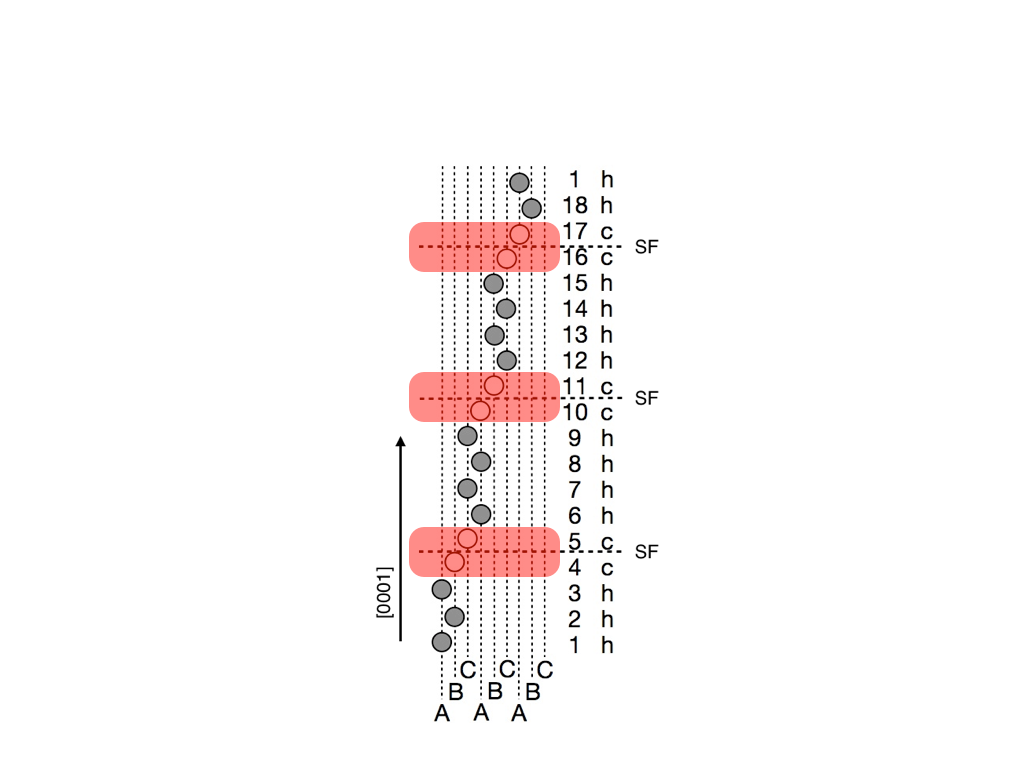
\includegraphics[width=63mm]{lpso.png}
\caption{LPSO構造の模式図.}
\label{default}
\end{center}
\end{figure}

\section{手法}
清原らは,L1$_2$クラスターを母相のMgがとるhcp構造に強引に導入すると,2つに分裂したより小さなclusterが生成すると予測している\cite{kiyohara}.
このサイズは小角散乱の実験から奥田らが報告しているクラスターサイズに近い\cite{okuda}.

このsmall clusterをL1$_2$ クラスターから1層ずつ離れた位置に挿入して, VASP を用いて第一原理計算を行い構造緩和したエネルギーを求める. VASP で計算を行う場合, 無限周期の固体を考えなければならないが計算モデル内の原子が増えるにつれ計算時間も増えるため, 無限周期のモデルの計算を行うことはできない. そこで同じモデルが全方向に無限に隣接したようなモデルを考える.このような計算条件を周期的境界条件という.
本研究で行う構造緩和は,結晶中の各原子を個々に移動させる内部緩和と,格子定数を変化させて結晶格子の構造自体を緩和させる外部緩和を用いて,最安定構造を求め,エネルギー値を算出する.



\section{考察}
上下に分割した際の small cluster の生成エネルギーが低く,安定構造となった.
上下に分割したsmall clusterを,積層欠陥にあるL1$_2$ クラスターから離れた位置へ図 2 に示したように挿入した. 
第一原理計算によって得られた系全体のエネルギーを図 3 に示した. 4 層離れた位置での計算についてはエネルギー値が収束していないが,他の層の計算結果から 距離が離れるに連れ単調減少を示すだけでなく,僅かではあるが中距離に安定位置がある傾向を示している. 



\begin{figure}
    \begin{tabular}{cc}
      \begin{minipage}{0.5\hsize}
        \centering
        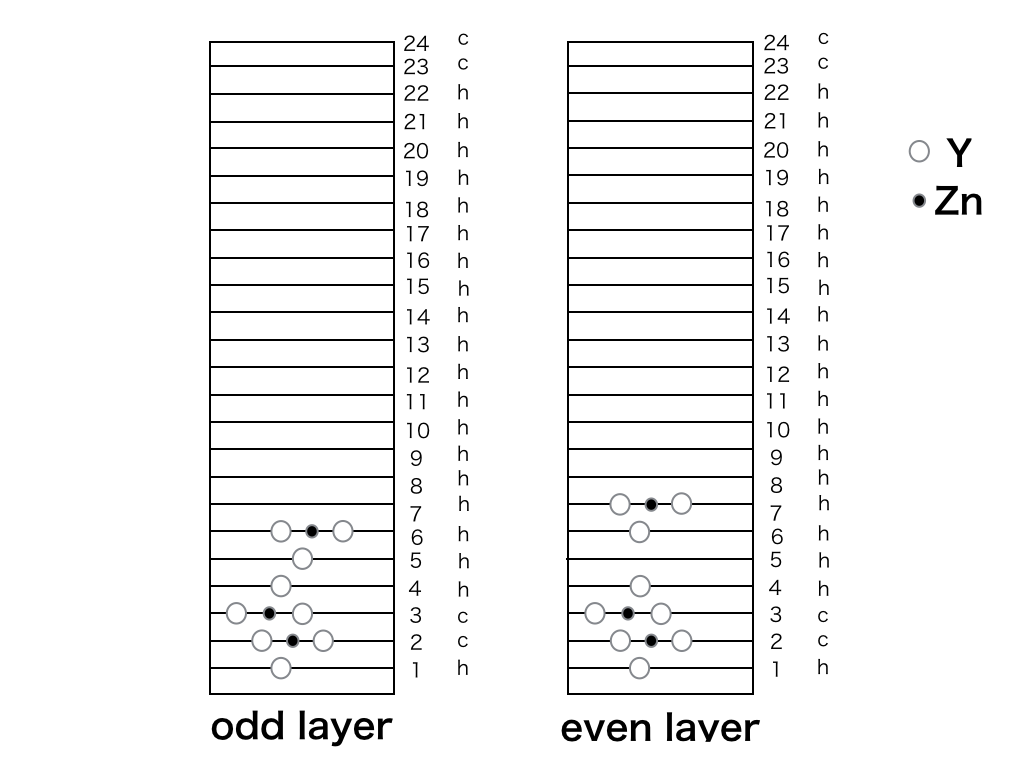
\includegraphics[width=45mm]{small_cluster_slab.png}
        \caption{計算モデルの模式図.}
        \label{default}
      \end{minipage} &
      \begin{minipage}{0.5\hsize}
        \centering
        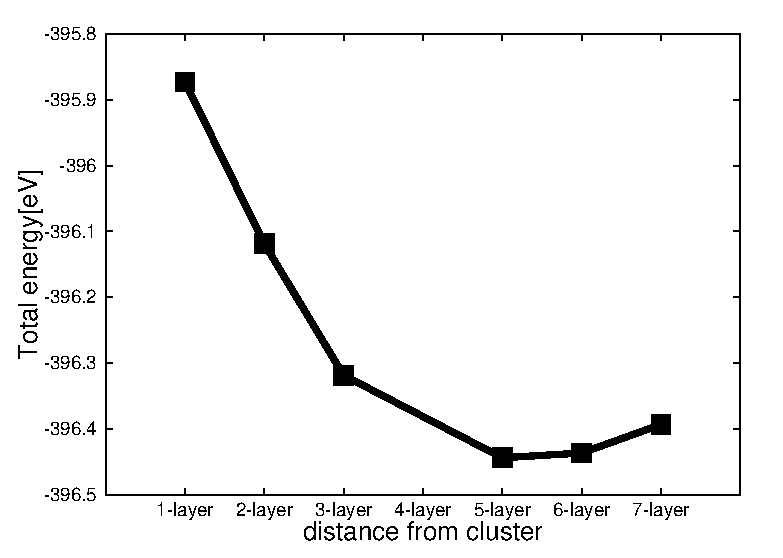
\includegraphics[width=45mm]{small_cluster.eps}
        \caption{L1$_2$ クラスターと small cluster の距離による エネルギー変化.}
        \label{default}
      \end{minipage}
    \end{tabular}
  \end{figure}

\section{今後の研究}
今後は,4層離れた位置での計算が収束に向かうよう分析し, より遠くの離れた積層まで入れる.
また、現段階では small cluster をL1$_2$クラスターの真上の位置に置いているが、 small cluster を違う位置に置いたモデルについても計算を行う.


\begin{thebibliography}{9}
\bibitem{kiyohara} M. Kiyohara, Y. Sakamoto, T. Yoshioka, S. Morishita, and S. R. Nishitani: proceedings of PRICM9, (Kyoto 2016).

\bibitem{sakamoto}Y. Sakamoto, C. Shirayama, Y. Yamamoto, R. Kubo, M. Kiyohara, and S. R. Nishitani: Mater. Trans., {\bf 56}(2015), 933.

\bibitem{okuda} H. Okuda, M. Yamasaki, Y. Kawamura, M. Tabuchi, H. Kimizuka: Scientific Reports, {\bf5} (2015), 14186.
\end{thebibliography}


\end{document}